\documentclass{article}
\usepackage{neurips_2026}      % <-- for submission, replace with the OFFICIAL NeurIPS 2026 style
\usepackage[utf8]{inputenc}
\usepackage[T1]{fontenc}
\usepackage{hyperref}
\usepackage{url}
\usepackage{booktabs}
\usepackage{amsmath}
\usepackage{tikz}
\usetikzlibrary{arrows.meta,positioning,fit,backgrounds}
\hypersetup{colorlinks=true,linkcolor=black,citecolor=black,urlcolor=blue}

\title{A Judge That Cannot Certify Itself:\\ A Code-Enforced Trust Protocol for Adversarial LLM Auditing}

\author{%
  Anonymous Author(s)\\
  Affiliation withheld for double-blind review\\
  \texttt{email withheld}%
}

\begin{document}
\maketitle

\begin{abstract}
LLM-based evaluators fail most dangerously when they are \emph{reliable without being valid}:
internally consistent, confident, and biased. The largest systematic study of LLM-as-a-judge to date
reports exactly this dissociation---test--retest consistency above $0.95$ coexisting with severe
position bias, and exact-match agreement overstating discrimination by $33$--$41$ points of $\kappa$
once chance-corrected~\cite{norman2026reliability}. Such a judge is at its most harmful the moment it is
allowed to \emph{certify itself}---to declare its own output validated, or to count its own internal
agreement as independence. We present a \emph{trust protocol}: a small set of invariants an adversarial
LLM-audit pipeline is made to obey \emph{in ordinary code}, not in prompts, and each pinned by a test.
(1)~The pipeline can never return \textsc{Validated} on internal grounds; human closure is a
\emph{cryptographic} HMAC of the audit-ledger digest under a key the model cannot reach, so a model that
authors the payload cannot sign its own validation. (2)~Cross-model independence is \emph{attested by the
calling adapter}, not read from a self-report. (3)~A run is admitted only under an \emph{A+B contract}---a
\emph{measured} minimum of layers actually executed \textbf{and} every other layer carries an explicit
applicable/not-applicable verdict---otherwise the pipeline \emph{refuses to close} and exits non-zero, a
refusal that overrides even a valid human attestation. (4)~The engine is turned on itself and the audit
trail is shipped, including a different-vendor review that overturned an earlier version of our own
central empirical claim. We make \textbf{no detection-superiority claim}; the contribution is the closure
discipline itself, and a per-run \emph{disclosure record}---which layers ran, which were adjudicated out
and why, what independence was attested, whether closure was reached---that a judge cannot silently
violate. This is a machine-checked instance of the judge-deployment disclosure standard JUDGe is
convening~\cite{judge2026}.
\end{abstract}

\section{The problem: self-certification, not inaccuracy}
Evaluation validity is a property of a judge \emph{in a system}, not in isolation~\cite{judge2026}. A
well-calibrated judge can fail systematically once its output gates a safety decision or feeds back into
training. The specific failure we target is \emph{self-certification}: a judge that treats its own
stability as validity and its own agreement as independence. Norman et al.~\cite{norman2026reliability}
supply the empirical warrant---across $21$ judges from nine providers and roughly $541{,}000$ individual
judgments, reliability and validity are dissociated---but a diagnosis is not a mechanism. If a
biased-but-consistent judge can stamp its own output ``validated,'' everything downstream inherits an
error the system cannot see. The question we take up is not \emph{how accurate is the judge} but
\emph{can the judge be stopped from closing its own loop}.

\section{The protocol}
The system is an orchestrator that spawns adversarial LLM sub-agent roles (an oracle that cites facts and
emits no verdicts; a verifier that recomputes and, where code is runnable, \emph{executes} it; a
propagator that constructs the concrete sequence violating a guarantee) and hands their findings to a
\emph{deterministic core} that assigns verdicts and decides completion. The orchestrator coordinates; it
does not judge (Figure~\ref{fig:bands}). Four invariants live in that core.

\begin{figure}[t]
\centering
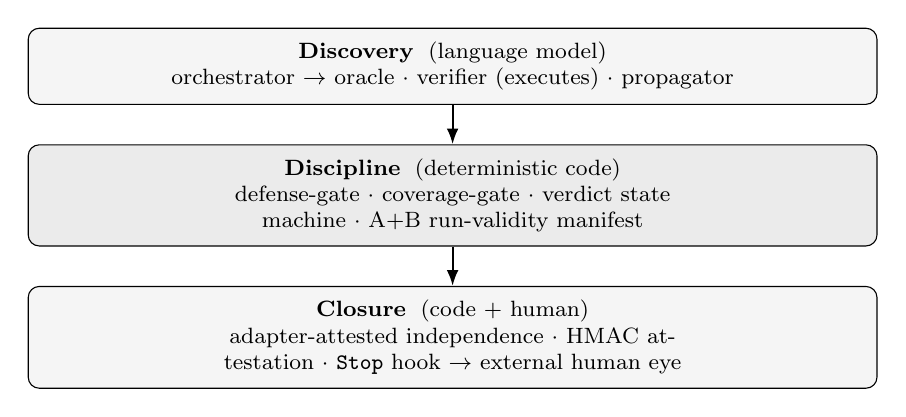
\begin{tikzpicture}[
  font=\footnotesize,
  band/.style={draw, rounded corners, align=center, inner sep=5pt, minimum height=8mm},
  arr/.style={-{Latex[length=2mm]}, thick}]
  \node[band, fill=black!4, text width=0.86\linewidth] (disc)
    {\textbf{Discovery} \;(language model)\\ orchestrator $\to$ oracle $\cdot$ verifier (executes) $\cdot$ propagator};
  \node[band, fill=black!8, below=5mm of disc, text width=0.86\linewidth] (disp)
    {\textbf{Discipline} \;(deterministic code)\\ defense-gate $\cdot$ coverage-gate $\cdot$ verdict state machine $\cdot$ A+B run-validity manifest};
  \node[band, fill=black!4, below=5mm of disp, text width=0.86\linewidth] (clos)
    {\textbf{Closure} \;(code $+$ human)\\ adapter-attested independence $\cdot$ HMAC attestation $\cdot$ \texttt{Stop} hook $\to$ external human eye};
  \draw[arr] (disc) -- (disp);
  \draw[arr] (disp) -- (clos);
\end{tikzpicture}
\caption{Three bands. Fallibility lives in the language-model band; \emph{discipline and trust live in
ordinary code}. The core assigns verdicts and decides closure; it can refuse, but it cannot self-certify.}
\label{fig:bands}
\end{figure}

\paragraph{I1 --- Non-closure is cryptographic.} The completion state machine reaches \textsc{Validated}
only on a valid HMAC of the ledger digest under an operator key held outside the model's reach. A bare
``human-approved'' token that does not verify closes nothing. A \texttt{Stop} hook re-verifies the HMAC
in the operator's environment and, if a \textsc{Validated} does not verify, downgrades the ledger on
disk. The model authors the payload but not the key: it cannot forge its own validation.

\paragraph{I2 --- Independence is attested, not claimed.} Different-vendor review is credited
(independence level~3) only from the identity the \emph{calling adapter} reports. A different-vendor
label present only in the payload is recorded as \textsc{Cross\_Model\_Claimed} and buys no independence
credit. This directly answers the self-preference / correlated-blind-spot facet: a second model prompted
adversarially by the same vendor is not counted as an independent draw.

\paragraph{I3 --- The A+B run-validity contract.} A pipeline that silently skips layers can still print
a confident verdict; the danger is a run that \emph{looks} complete because no one counted what did not
happen. A run is admitted only if \textbf{(A)}~a measured minimum of required layers actually
executed---measured from each layer's own output, not from self-report---\textbf{and (B)}~every other
layer carries an explicit \textsc{Ran}/\textsc{Not\_Applicable}/\textsc{Missing} status with
justification. The manifest computes \texttt{run\_validity}; if it is not \textsc{Valid}, completion is
forced to \textsc{Invalid\_Run}, which \emph{overrides every other state, including a valid human}
\textsc{Validated}, and the process exits non-zero. Closure cannot be bought by signing an incomplete
process. The required minimum was itself \emph{measured} across ten runs over eight artifact classes, not
assumed---and the measurement corrected an earlier over-inclusion (one role frozen as required was
returned to optional once two classes reached their defects without it).

\paragraph{I4 --- Self-audit, shipped.} The engine is run against its own artifacts and papers and the
ledgers are committed. This is not decoration: a same-vendor self-audit (independence level~1) located
four defects in our own closure guarantees; a later different-vendor review (level~3) overturned the
original headline empirical claim and forced two guarantees from convention into cryptographic code; and
the measurement instrument of I3, when first run, found three real defects \emph{in itself}. We report
these because a system whose value is adversarial honesty must show the audits that caught it.

Each invariant is a test in a $173$-test suite run in CI across Python 3.10--3.13, including an
end-to-end step that \emph{fails if the pipeline ever prints} \textsc{Validated} \emph{without a human}.

\begin{figure}[t]
\centering
\fbox{\begin{minipage}{0.92\linewidth}\footnotesize\ttfamily
run\_validity : VALID\hfill \# A+B contract satisfied\\
completion~~~ : EXTERNAL\_REVIEW\_PENDING\hfill \# no attested external identity $\to$ not validated\\
layers~~~~~~~ : triage=RAN~ oracle=RAN~ verifier=RAN~ propagator=RAN~ governor=RAN\\
\phantom{layers~~~~~~~ : }reasoner=NOT\_APPLICABLE\hfill \# not selected by triage\\
\phantom{layers~~~~~~~ : }deep\_causal=NOT\_APPLICABLE\hfill \# not selected by triage\\
\phantom{layers~~~~~~~ : }external\_auditor=NOT\_APPLICABLE\hfill \# not selected by triage\\
source\_grade : \{primary:2, institutional:0, generalist:0, unknown:0\}
\end{minipage}}
\caption{A per-run \emph{disclosure record} --- verbatim output of \texttt{run\_core.py} on a complete
run. It states which layers ran, which were adjudicated out and \emph{why}, that the A+B contract holds
(\textsc{Valid}), and that closure was \emph{not} reached because no external identity was attested. This
is a machine-checked instance of the disclosure JUDGe is convening; the pipeline refuses to close when
the record is incomplete.}
\label{fig:disclosure}
\end{figure}

\paragraph{Reproducibility and artifact.} The system is an MIT-licensed engine with four reproducible
benchmarks and the $173$-test suite above. From a clone, \texttt{python3 -m unittest discover -s tests}
and \texttt{reproduce.py -{}-strict} on each benchmark recompute every quantitative claim to the digit;
the disclosure record of Figure~\ref{fig:disclosure} is the verbatim output of \texttt{run\_core.py}. An
anonymized copy of the repository is provided for review so that reviewers can clone it and run the
gates, the refusal, and the cryptographic-closure check themselves; the public repository is disclosed on
acceptance.

\section{Relation to existing work}
\paragraph{Reliability vs.\ validity of judges.} \cite{norman2026reliability} is the motivation and the
missing-enforcement counterpart: they measure that judges are reliable-without-valid and recommend a
``Minimum Viable Validation Protocol,'' but a recommendation is advisory---a judge can decline it and
certify itself anyway. We make the most dangerous consequence, self-certification, structurally
impossible in code. We do not re-measure judge bias.

\paragraph{Adversarial defect discovery.} The closest adversarial system,
Refute-or-Promote~\cite{agarwal2026refute}, shares the adversarial kill-mandate and a cross-model critic
and demonstrates them at scale (a 31-day campaign, ${\sim}171$ candidates, ${\sim}79\%$ killed before
disclosure, real CVEs and accepted ISO~C++ defect reports). We claim no priority on those ideas. The
difference is the objective: Refute-or-Promote optimizes \emph{precision of discovery} with a human
orchestrator and no enforced non-closure---its cross-model step \emph{improves} reliability but nothing
\emph{forbids} a confident close. We optimize \emph{trustworthiness of closure}: judging is code,
independence must be adapter-attested, closure is cryptographic, and an under-run is refused
non-bypassably. A better \emph{finder} versus a \emph{finder that cannot lie about having finished}; the
two are complementary.

\paragraph{Adversarial robustness of judges.} Work on prompt-injection attacks against
judges~\cite{maloyan2025adversarial} asks whether a judge can be \emph{fooled from outside}. We ask the
orthogonal question---whether a judge can be \emph{stopped from certifying itself from inside}---and
enforce the answer in code rather than in a prompt.

\paragraph{JUDGe's disclosure template.} The workshop's community deliverable is a judge-deployment
disclosure standard (provenance, deployment context, known failure modes, human
validation)~\cite{judge2026}. Our execution manifest and A+B record are a \emph{machine-checked instance}
of such a disclosure: emitted per run, refused when incomplete.

\section{Limitations}
We make no detection-superiority claim; a small-sample study behind this system (seven real errors, one
run per model nature) is a descriptive dissociation, not a recall result, and is reported as such in the
companion systems paper. The cryptographic non-closure is only as strong as the operator's key
hygiene---it contracts forgery from a payload field to an out-of-band secret, it does not eliminate it.
Real cross-vendor independence depends on an adapter the operator must wire up; absent it, the
external-auditor role is theatre, and the code says so. And the whole apparatus is a \emph{survivor}:
every internal audit sits at independence level $\leq 3$ in a single lab and validates nothing---by
construction, only an external human eye closes the loop. That is the protocol's own thesis applied to
itself.

\begin{thebibliography}{9}
\bibitem{norman2026reliability}
J.~D. Norman, M.~U. Rivera, and D.~A. Hughes.
\newblock Reliability without Validity: A Systematic, Large-Scale Evaluation of LLM-as-a-Judge Models
Across Agreement, Consistency, and Bias.
\newblock arXiv:2606.19544, 2026.

\bibitem{agarwal2026refute}
A.~Agarwal.
\newblock Refute-or-Promote: An Adversarial Stage-Gated Multi-Agent Review Methodology for
High-Precision LLM-Assisted Defect Discovery.
\newblock arXiv:2604.19049, 2026.

\bibitem{maloyan2025adversarial}
N.~Maloyan and D.~Namiot.
\newblock Adversarial Attacks on LLM-as-a-Judge Systems: Insights from Prompt Injections.
\newblock arXiv:2504.18333, 2025.

\bibitem{judge2026}
JUDGe @ NeurIPS 2026.
\newblock Can We Trust the Judge? Workshop call for papers and failure taxonomy.
\newblock \url{https://judge2026.github.io/}, 2026.
\end{thebibliography}

\vfill
\begin{center}\footnotesize
Anonymized for double-blind review. Artifact (MIT-licensed engine; four reproducible benchmarks; 173
tests; CI-checked protocol invariants) available at an anonymized repository; de-anonymized on
acceptance.
\end{center}

\end{document}
